\documentclass{article}
\usepackage{listings}
\usepackage{xcolor}
\usepackage[margin=1in]{geometry}
\usepackage{amsmath,amsthm,amssymb}
\usepackage{graphicx}
\usepackage{epstopdf}
\DeclareGraphicsExtensions{.eps,.ps,.jpg,.bmp}
\lstset{
	numbers=left,
    framexleftmargin=10mm,
    frame=none,
    backgroundcolor=\color[RGB]{245,245,244},
	keywordstyle=\bf\color{blue},
	identifierstyle=\bf,
	numberstyle=\color[RGB]{0,192,192},
	commentstyle=\it\color[RGB]{0,96,96},
	stringstyle=\rmfamily\slshape\color[RGB]{128,0,0},
	showstringspaces=false
    }

\newcommand{\N}{\mathbb{N}}
\newcommand{\R}{\mathbb{R}}
\newcommand{\Z}{\mathbb{Z}}
\newcommand{\Q}{\mathbb{Q}}

\newenvironment{theorem}[2][Theorem]{\begin{trivlist}
\item[\hskip \labelsep {\bfseries #1}\hskip \labelsep {\bfseries #2.}]}{\end{trivlist}}
\newenvironment{lemma}[2][Lemma]{\begin{trivlist}
\item[\hskip \labelsep {\bfseries #1}\hskip \labelsep {\bfseries #2.}]}{\end{trivlist}}
\newenvironment{exercise}[2][Exercise]{\begin{trivlist}
\item[\hskip \labelsep {\bfseries #1}\hskip \labelsep {\bfseries #2.}]}{\end{trivlist}}
\newenvironment{problem}[2][Problem]{\begin{trivlist}
\item[\hskip \labelsep {\bfseries #1}\hskip \labelsep {\bfseries #2.}]}{\end{trivlist}}
\newenvironment{question}[2][Question]{\begin{trivlist}
\item[\hskip \labelsep {\bfseries #1}\hskip \labelsep {\bfseries #2.}]}{\end{trivlist}}
\newenvironment{corollary}[2][Corollary]{\begin{trivlist}
\item[\hskip \labelsep {\bfseries #1}\hskip \labelsep {\bfseries #2.}]}{\end{trivlist}}

\begin{document}

\title{Homework 2016-03-23}
\author{Chuan Lu\\
13300180056}

\maketitle

\begin{problem}{1}
\text{ }\\
Solve the ODE $\frac{du}{dt} = u - u^{3}$ with Taylor series iteration.
\end{problem}

\begin{proof}
\subsection{The code is shown as follows.} 
\begin{lstlisting}[language={MATLAB}]
function [t, u] = Taylor_iter(func, inteval, u0, delta_t, order, F, G)
% TAYLOR_ITER The main function of Taylor series Iteration of solving ODEs
% The equation behave likes du/dt = f(t, u), with initial condition given 
% as u(0) = u0 in the inteval [a, b];

% input:
% func : a function of two variables t, u;
% inteval : a list of the inteval of the equation, given like [a, b];
% u0 : the initial condition;
% delta_t : the step size of time;
% order : the order of the iteration, chosen from {1, 2, 3};
% F : needed if the order = 2; 
% G: needed if the order = 3;

% output:
% t : the list of time, inited by the inteval and delta_t;
% u : the value of u at the points in t;

if nargin < 2
    error('More arguments needed --Taylor-iter');
elseif nargin == 2
    u0 = 1;
    delta_t = 1/8;
    order = 1;
elseif nargin == 3
    delta_t = 1/8;
    order = 1;
elseif nargin == 4
    order = 1;
end

if order == 2
    if nargin <= 5
        error('F is needed --Taylor-iter');
    end
elseif order == 3
    if nargin <= 6
        error('G is needed --Taylor-iter');
    end
end

if length(inteval) ~= 2 || inteval(1) >= inteval(2)
    error('Invalid inteval --Taylor-iter');
end

switch order
    case 1
        [t, u] = explicit_iter(func, inteval, u0, delta_t);
    case 2
        [t, u] = taylor_iter_2order(func, F, inteval, u0, delta_t);
    case 3
        [t, u] = taylor_iter_3order(func, F, G, inteval, u0, delta_t);
    otherwise
        error('Invalid order --Taylor-iter');
end
\end{lstlisting}

\begin{lstlisting}[language={MATLAB}]
function [ t, u ] = explicit_iter( func, inteval, u1, delta_t )
% EXPLICIT_ITER Explicit Euler Iteration

t = inteval(1):delta_t:inteval(2);
n = length(t);
u = zeros(1, n);

for i = 1 : n
    u(i) = u1;
    u1 = u1 + delta_t * feval(func, t(i), u(i));
end
\end{lstlisting}

\begin{lstlisting}[language={MATLAB}]
function [t, u] = taylor_iter_2order(func, F, inteval, u1, delta_t)
%TAYLOR_ITER_2ORDER The 2nd-order taylor iteration

t = inteval(1):delta_t:inteval(2);
n = length(t);
u = zeros(1, n);

for i = 1:n
    u(i) = u1;
    delta = feval(func, t(i), u(i)) + feval(F, t(i), u(i))*delta_t/2;
    u1 = u1 + delta_t * delta;
end
\end{lstlisting}

\begin{lstlisting}[language={MATLAB}]
function [t, u] = taylor_iter_3order(func, F, G, inteval, u1, delta_t)
%TAYLOR_ITER_3ORDER The 3rd-order taylor iteration

t = inteval(1):delta_t:inteval(2);
n = length(t);
u = zeros(1, n);

for i = 1:n
    u(i) = u1;
    delta1 = feval(func, t(i), u(i)) + feval(F, t(i), u(i))*delta_t/2;
    delta2 = feval(G, t(i), u(i))*(delta_t^2)/6;
    u1 = u1 + (delta1 + delta2) * delta_t;
end
\end{lstlisting}

\begin{lstlisting}[language={MATLAB}]
% Page 74, Exercise 1
% solve du/dt = u - u^2;

func = @(t, u)(u - u .^ 2);
u0 = 1.5;
ui = 0.5;
inteval = [0, 8];
delta_t = 1/8;

order1 = 1;
order2 = 2;
order3 = 3;
order4 = 4;

F = @(t, u)((1-2.*u).*(u-u.^2));
G = @(t, u)((u-u.^2).*(6*u.^2-6*u+1));

[t, u1] = Taylor_iter(func, inteval, u0, delta_t, order1);
plot(t, u1, '*-');
hold on

[t2, u2] = Taylor_iter(func, inteval, u0, delta_t, order2, F);
plot(t2, u2, '.-');
hold on

[t3, u3] = Taylor_iter(func, inteval, u0, delta_t, order3, F, G);
plot(t3, u3, 'd-');
hold on

exact_func = @(x, u0)(1 ./ ((1/u0 - 1) .* exp(-x) + 1));
exact_value = feval(exact_func, t, u0);
plot(t, exact_value, '-');
hold on

[t11, u11] = Taylor_iter(func, inteval, ui, delta_t, order1);
plot(t11, u11, '*-');
hold on

[t21, u21] = Taylor_iter(func, inteval, ui, delta_t, order2, F);
plot(t21, u21, '.-');
hold on

[t31, u31] = Taylor_iter(func, inteval, ui, delta_t, order3, F, G);
plot(t31, u31, 'd-');
hold on

exact_value1 = feval(exact_func, t, ui);
plot(t, exact_value1, '-');

legend('Explicit Euler', '2nd-order Taylor', '3rd-order Taylor',...
    'Exact', 'Explicit Euler2', '2nd-order Taylor2',...
    '3rd-order Taylor2', 'Exact2', 'Location', 'Best');
title({['Solving du/dt = u-u^2 using Explicit Euler and 2/3-order'];
       ['Taylor iteration']});
grid on;
\end{lstlisting}

\subsection{The result is shown as follows.}
\begin{figure}[htbp]
\centering
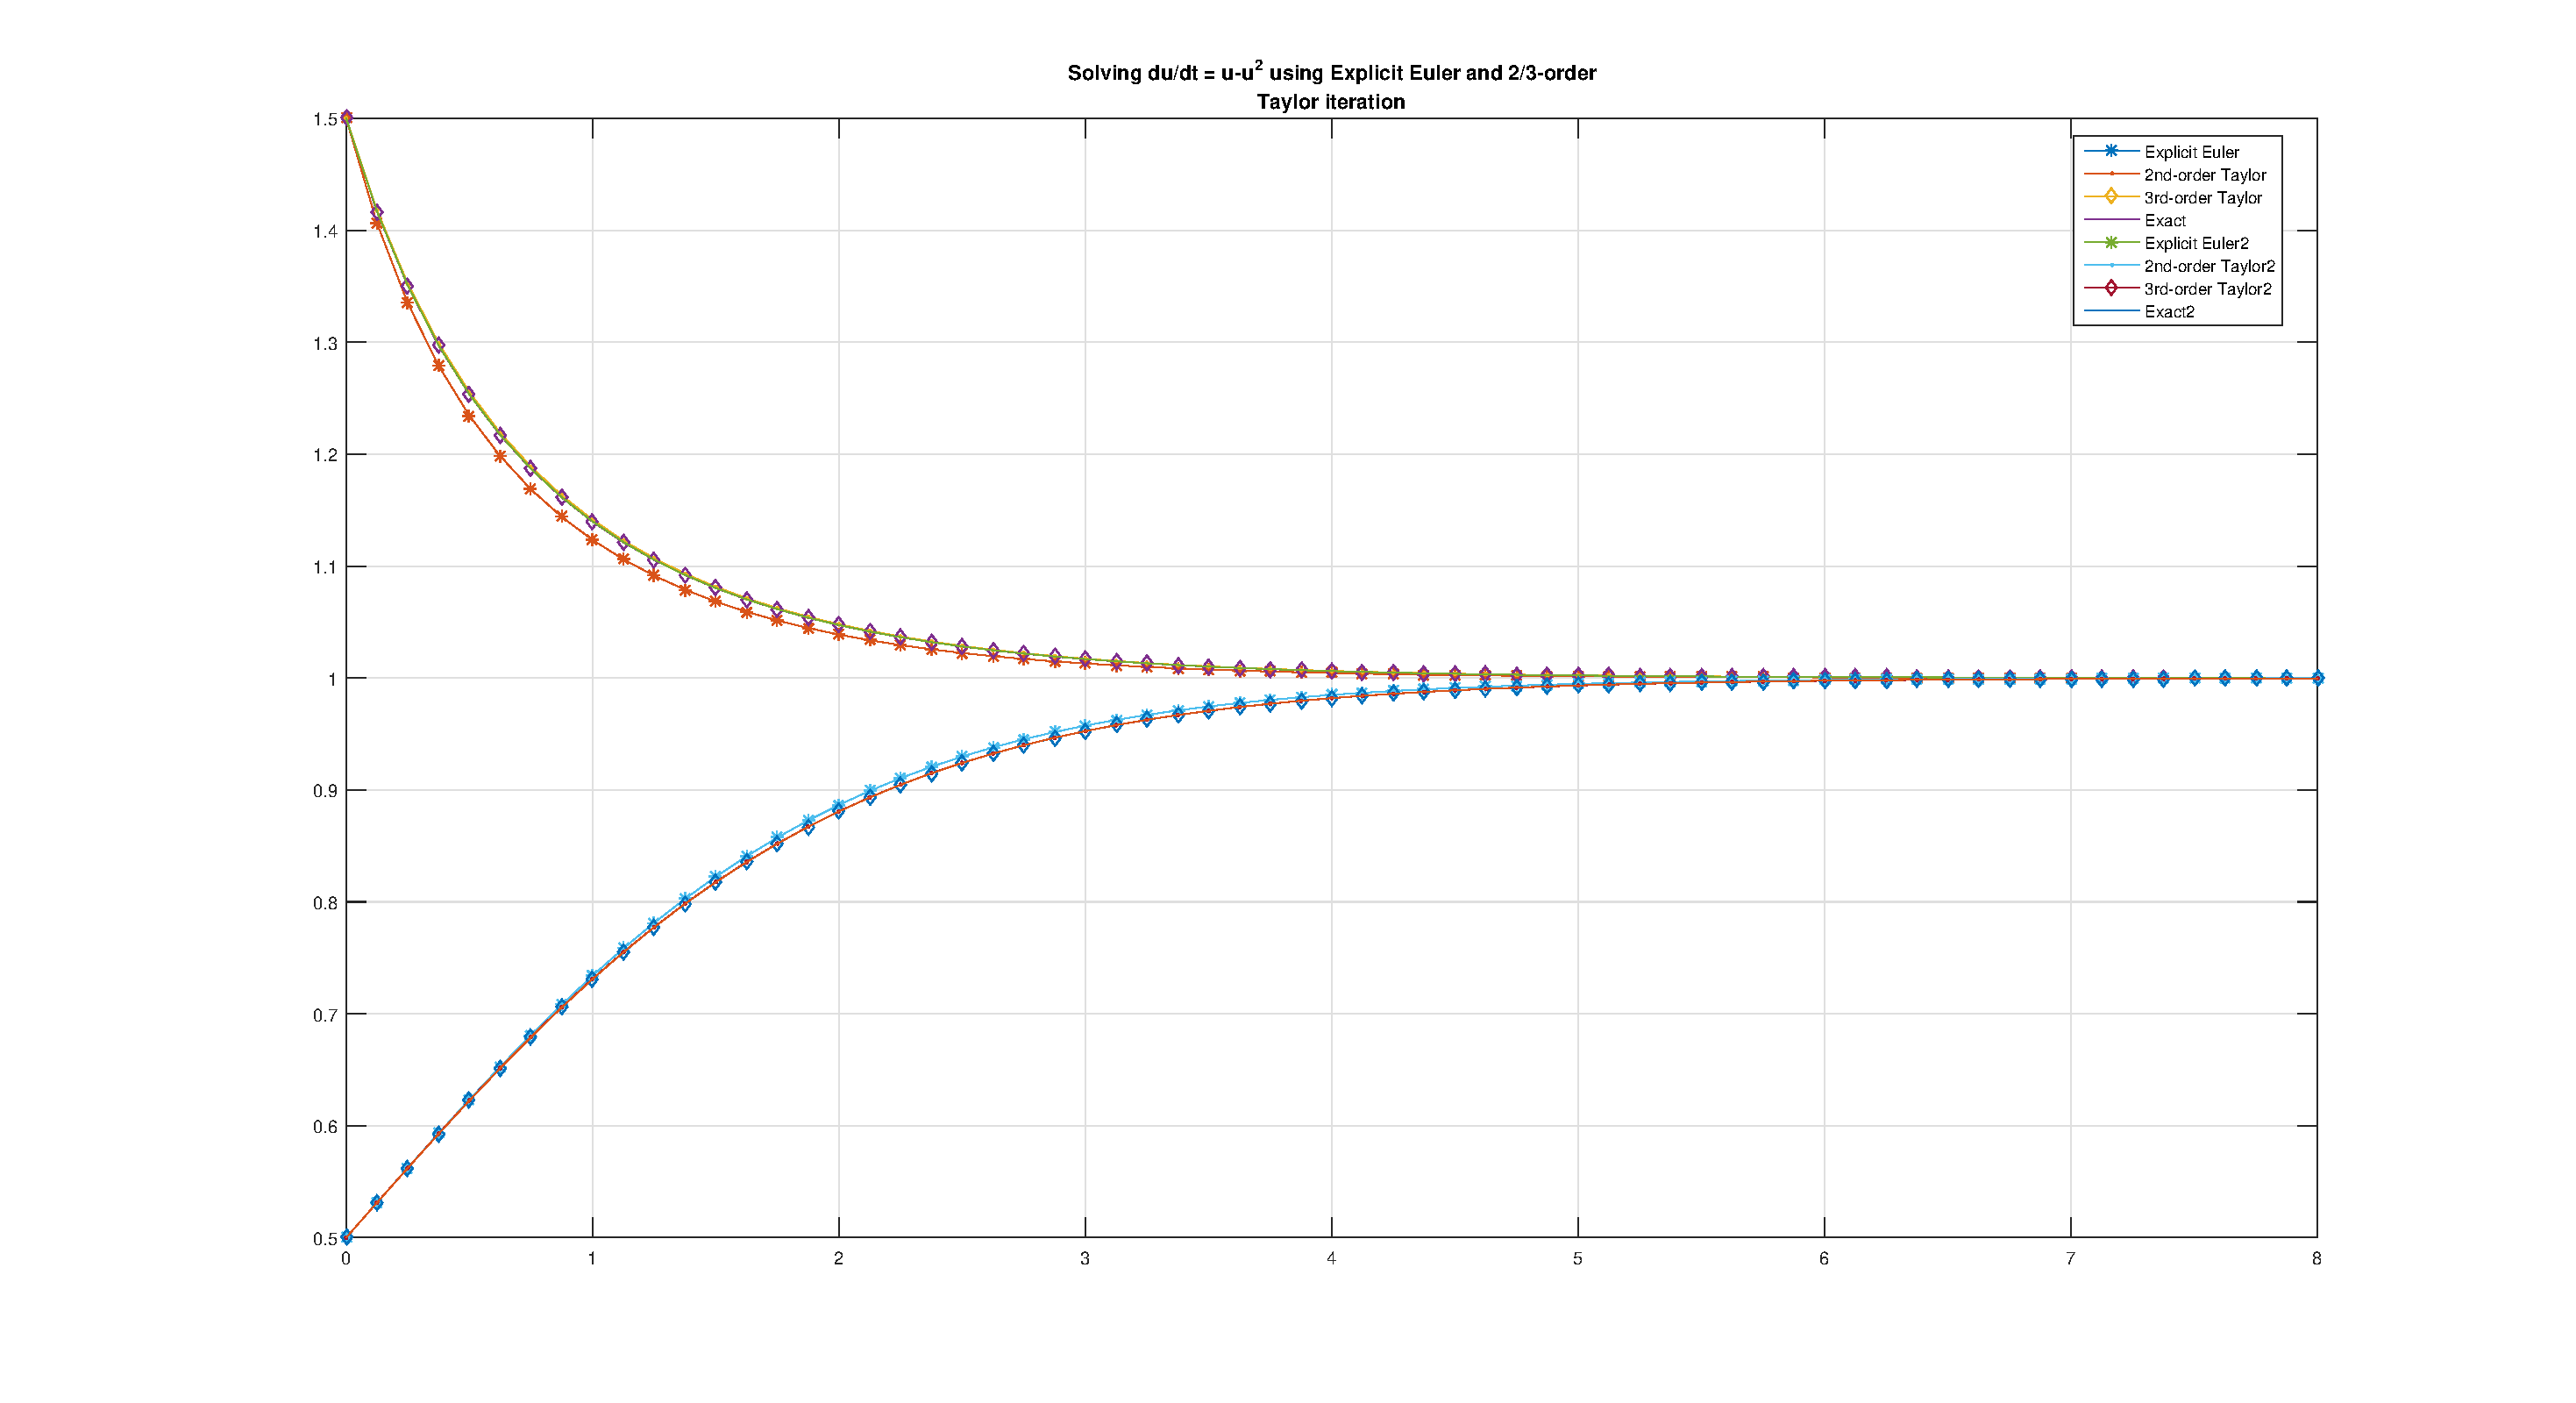
\includegraphics[width = 15cm]{solve.eps}
\caption{The solvation with Taylor series iteration.}
\label{Solve}
\end{figure}
\end{proof}

\begin{problem}{2}
\text{ }\\
Draw the convergence order of Runge-Kutta iteration.
\end{problem}
\begin{proof}
\subsection{The code is shown as follows.}
\begin{lstlisting}[language = {MATLAB}]
function [t, u] = Runge_Kutta(func, inteval, u0, delta_t, order)
% RUNGE_KUTTA The main function of Runge Kutta Iteration of solving ODEs
% The equation behave likes du/dt = f(t, u), with initial condition given 
% as u(0) = u0 in the inteval [a, b];

% input:
% func : a function of two variables t, u;
% inteval : a list of the inteval of the equation, given like [a, b];
% u0 : the initial condition;
% delta_t : the step size of time;
% order : the order of the iteration, chosen from {1, 2, 3, 4};

% output:
% t : the list of time, inited by the inteval and delta_t;
% u : the value of u at the points in t;


if nargin < 2
    error('More arguments needed --Runge-Kutta');
elseif nargin == 2
    u0 = 1;
    delta_t = 1/8;
    order = 1;
elseif nargin == 3
    delta_t = 1/8;
    order = 1;
elseif nargin == 4
    order = 1;
end

if length(inteval) ~= 2 || inteval(1) >= inteval(2)
    error('Invalid inteval --Runge-Kutta');
end

switch order
    case 1
        [t, u] = explicit_iter(func, inteval, u0, delta_t);
    case 2
        [t, u] = Kutta_2order(func, inteval, u0, delta_t);
    case 3
        [t, u] = Kutta_3order(func, inteval, u0, delta_t);
    case 4
        [t, u] = Kutta_4order(func, inteval, u0, delta_t);
    otherwise
        error('Invalid order --Runge-Kutta');
end
\end{lstlisting}

\begin{lstlisting}[language = {MATLAB}]
function [ t, u ] = explicit_iter( func, inteval, u1, delta_t )
% EXPLICIT_ITER Explicit Euler Iteration

t = inteval(1):delta_t:inteval(2);
n = length(t);
u = zeros(1, n);

for i = 1 : n
    u(i) = u1;
    u1 = u1 + delta_t * feval(func, t(i), u(i));
end
\end{lstlisting}

\begin{lstlisting}[language = {MATLAB}]
function [t, u] = Kutta_2order(func, inteval, u1, delta_t)
% Kutta_2order The 2nd-order Runge-Kutta iteration

t = inteval(1):delta_t:inteval(2);
n = length(t);
u = zeros(1, n);

for i = 1:n
    u(i) = u1;
    delta1 = u(i) + delta_t * feval(func, t(i), u(i));
    delta2 = feval(func, t(i) + delta_t, delta1);
    u1 = u1 + delta_t / 2 * (feval(func, t(i), u(i)) + delta2);
end
\end{lstlisting}

\begin{lstlisting}[language = {MATLAB}]
function [t, u] = Kutta_3order(func, inteval, u1, delta_t)
% Kutta_3order The 3rd-order Runge-Kutta iteration

t = inteval(1):delta_t:inteval(2);
n = length(t);
u = zeros(1, n);

for i = 1:n
    u(i) = u1;
    delta1 = feval(func, t(i), u(i));
    delta2 = feval(func, t(i)+delta_t/2, u(i)+delta_t/2*delta1);
    delta3 = feval(func, t(i)+delta_t, u(i)-delta_t*delta1+2*delta_t*delta2);
    u1 = u1 + delta_t/6*(delta1 + 4*delta2 + delta3);
end
\end{lstlisting}

\begin{lstlisting}[language = {MATLAB}]
function [t, u] = Kutta_4order(func, inteval, u1, delta_t)
% Kutta_4order The 4th-order Runge-Kutta iteration

t = inteval(1):delta_t:inteval(2);
n = length(t);
u = zeros(1, n);

for i = 1:n
    u(i) = u1;
    delta1 = feval(func, t(i), u(i));
    delta2 = feval(func, t(i)+delta_t/2, u(i)+delta_t/2*delta1);
    delta3 = feval(func, t(i)+delta_t/2, u(i)+delta_t/2*delta2);
    delta4 = feval(func, t(i)+delta_t, u(i)+delta_t*delta3);
    u1 = u1 + delta_t/6*(delta1 + 2*delta2 + 2*delta3 + delta4);
end
\end{lstlisting}

\begin{lstlisting}[language = {MATLAB}]
% Page 79, Exercise 3
figure(2)
symbol = {'*-', '.-', 'd-', 'o-'};
m = 13;
error_list = zeros(4, m);
for j = 1:m
    delta_t = 2 ^ (-j);
    t = inteval(1):delta_t:inteval(2);
    exact_value = feval(exact_func, t, u0);
    for i = 1:4
        [t, u] = Runge_Kutta(func, inteval, u0, delta_t, i);
        error_list(i, j) = max(abs(u - exact_value));
    end
end
for i = 1 : 4
    semilogy(1:1:13, error_list(i, :), cell2mat(symbol(i)));
    hold on;
end
legend('1st-order', '2nd-order', '3rd-order', '4th-order', 'Location',...
    'Best');
title('The absolute error of Runge-Kutta Iteration');
grid on;
\end{lstlisting}

\subsection{The result is shown as follows.}
\begin{figure}[htbp]
\centering
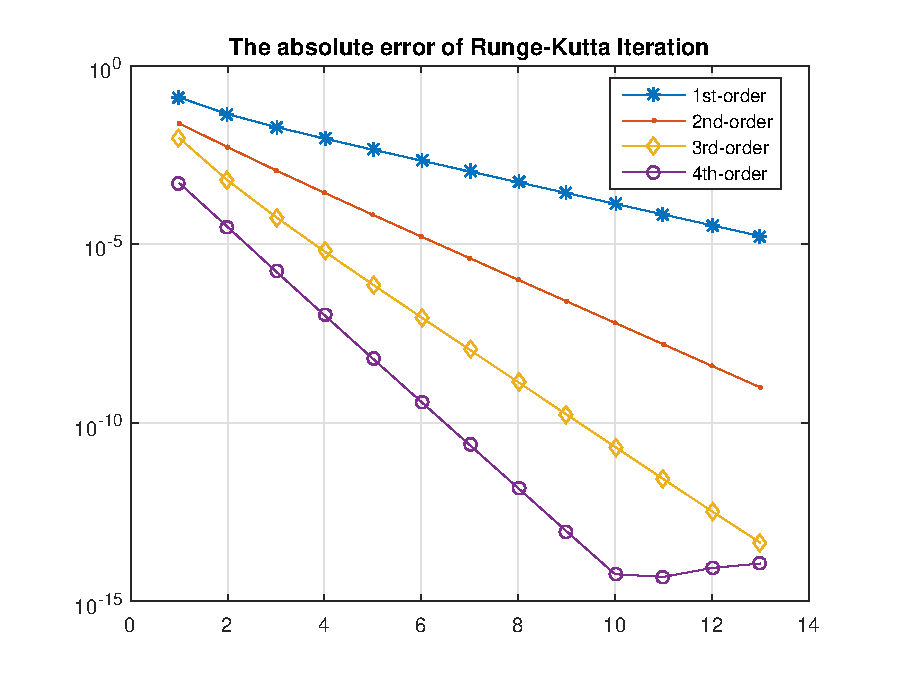
\includegraphics[width = 15cm]{errorlist.eps}
\caption{The convergence order of Runge-Kutta Iteration.}
\label{Convergence}
\end{figure}
\end{proof}
\end{document}
